\documentclass[]{article}
\usepackage{mathrsfs}
\usepackage{amsmath}
\usepackage{amsfonts}
\usepackage{graphicx}
\usepackage[left=20mm, right=20mm, top=20mm, bottom=20mm]{geometry}

\begin{document}
\huge Numeros complejos.
\\
\\
\Large Definición de un numero complejo.
\normalsize
\\
\\
Para empezar a hablar de numeros complejos primero hay que definir a la unidad imaginaria.
$$
\sqrt{-1} = i
$$
Todos los numeros de la forma $bi$ donde $b \in \mathbb{R}$ son numeros puramente imaginario.

Un numero complejo es la suma entre un numero real y uno imaginario y se suelen llamar $z$ tal que:
$$
z=a+bi
$$
Con $a \in \mathbb{R}$, $b \in \mathbb{R} $ y $z \in \mathbb{C}$
\\
\\
\Large Representación geometrica en el plano complejo
\normalsize
\\
\\
Los complejos pueden representarse en un plano mediante pares ordenados de numeros reales, esto se debe al isomorfismo que tiene $(\mathbb{C},+)$ con $(\mathbb{R}^{2},+)$ por lo tanto pueden representarse como vectores.

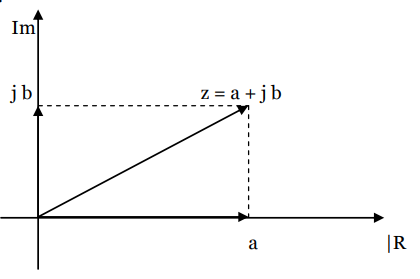
\includegraphics{../../../Imagenes/Superior/Complejos/Complejos01.PNG}


\Large Igualdad.
\normalsize
\\
\\
La igualdad entre numeros complejos se define asi:
$$
z_1 = a+bi \hspace{5pt}\wedge\hspace{5pt} z_2=c+di
$$
$$
z_1 = z_2 \Leftrightarrow a = c \hspace{5pt}\wedge\hspace{5pt} b = d
$$

\Large Modulo.
\normalsize
\\
\\
Geometricamente es el modulo del vector asociado a $z$.
$$
|z| = \sqrt{a^{2}+b^{2}}
$$

\Large Adición.
\normalsize
\\
\\
$$
z = z_1 +z_2 = a+bi + c+di = a+c+bi+di = (a+c) + (b+d) i
$$
Es equivalente a la suma de vectores, por lo tanto tiene sus mismas propiedades.
\Large Multiplicación.
\normalsize
\\
\\
$$
z = z_1 \cdot z_2 = (a+bi)\cdot(b+di) = (a\cdot c - b\cdot d) + i(a\cdot d + b \cdot c) 
$$
No es necesario recordar esta formula de memoria pues la suma es distributiva respecto de la multiplicación y se puede llegar al resultado operando con esta propiedad y recordando que $i^{2} = -1$.
\\
\\\\
\Large Conjugado.
\normalsize
\\
\\
El conjugado de un numero complejo $z=a+bi$ se define:
$$
\bar{z} = a - bi
$$
Es decir, tiene la misma parte real y opuesta parte imaginaria. El conjugado es distributiva respecto de la suma, multiplicación y división. Además hay una propiedad muy interesante que nos ayudará a resolver divisiones.
$$
z \cdot \bar{z} = |z|^{2}
$$
Esta propiedad es util para deshacerse de un denominador complejo multiplicando arriba y abajo por su conjugado similar a como se suele hacer con la radicación.
\\
\\
\Large Potencias naturales en forma Binomica
\normalsize
\\
\\
$$
z^{0} = 1
$$
$$
z^{1} = z
$$
$$
z^{n+1} = z^{n}\cdot z
$$
De acuerdo podemos calcular las potencias de la unidad imaginaria:
\begin{align}
  i^{0} &= 1 \\
  i^{1} &= i \\
  i^{2} &= -1 \\
  i^{3} &= -i \\
  i^{n} &= i^{r}
\end{align}
Siendo $r$ el resto de dividir a $n$ por $4$.
\\

Para poder calcular potencias en forma binomica $(a+bi)$ debemos utilizar el binomio de Newton:
$$
(a+bi)^{n} = \sum_{k=0}^{n}\binom{n}{k}a^{n-k}b^{k} 
$$
Esta sumatoria no es muy complicada de entender, tendremos $n$ terminos donde el coeficiente principal de cada uno está dado por el numero combinatorio entre $n$ y $k$. A medida que "avanzamos" en la sumatoria $k$ va aumentando de a $1$ haciendo que en cada termino la potencia de $b$ vaya aumentando hasta $n$ y la de $a$ disminuyendo desde $n$. No resulta de gran complejidad entender que está sucediendo y para llegar a las mismas conclusiones podemos tomar una potencia muy alta de un numero complejo y descomponerla en muchas multiplicaciones. Si intentamos generalizar ese proceso llegaremos al binomio de Newton. Una forma muy elegante de calcular complejos pero sin duda con demasiado trabajo. Mas adelante veremos como simplificar esta tarea.
\\
\\
\Large Raiz cuadrada en forma Binomica.
\normalsize
\\
\\

Diremos que $u$ es la raiz cuadradada de $z \Leftrightarrow z = u^{2}$  
Para esta operación realizaremos algunos calculos ya que no se puede ver a tan simple vista por donde comenzar.
\\
Sea $z = a+bi$ y $u = x + yi$:
\begin{align}
  u^{2}&= z\\
  (x+yi)^{2}&= a+bi\\
 x^{2}+2ixy-y^{2} &=a+bi\\
\end{align}
Por igualdad de complejos podemos deducir:
\begin{align}
  a &= x^{2} - y^{2}\\
  b &=2xy 
\end{align}
Por otro lado tambien podemos argumentar lo siguiente:
\begin{align}
  u^{2}&=z\\
  |u^{2}| &= |z|\\
  |u|^{2} &= |z|\\
  x^{2}+y^{2} &= |z| 
\end{align}
Si ahora sumamos miembro a miembro $(10)$ y $(15)$ obtenemos:
\begin{align}
  |z| + a &= 2x^{2}\\
  x &= \sqrt{\frac{|z|+a}{2}}  
\end{align}
Y si restamos miembro a miembro $(10)$ y $(15)$.
\begin{align}
|z| - a &= 2y^{2}\\
y &= \sqrt{\frac{|z|-a}{2}}  
\end{align}
Es decir: 
$$
u = \pm\sqrt{\frac{|z|+a}{2}}  \pm i\sqrt{\frac{|z|-a}{2}}   
$$
Lo cual nos dá como resultado $4$ posibles raices, pero sabemos que por el teorema fundamental del algebra, todo polinomio de grado $2$ tiene exactamente $2$ raices en el conjunto de los complejos.
\\ 
Podemos reestringir $2$ raices y dejarlas fuera gracias a la ecuación $(11)$. Recordemos que estamos calculando $\sqrt{z}$.
Los distintos valores de $u$ vienen dados por los signos de $x$ e $y$. Por la ecuación $(11)$ podemos ver que los mismos están ligados al signo de $b$. Es decir, si $x$ e $y$ tienen el mismo signo, entonces $b$ será positivo, si tienen distinto signo entonces $b$ será negativo. De esta forma podemos resolver la distorsión. Si $b$ es positivo tendremos dos soluciónes para $\sqrt{z}$, una donde $x$ e $y$ son positivos y otra donde $x$ e $y$ son negativos. Si $b$ es negativo aún tendremos dos soluciones pero en una de estas $x$ será positivo e $y$ negativo y en la otra $x$ será negativo e $y$ positivo.
\\
Observación: La formula resolvente es aplicable a complejos, siempre y cuando se realicen las operaciones como están definidas en el campo complejo.
\\

\huge Forma polar de un complejo.
\normalsize
\\
\\
Al igual que los vectores de $\mathbb{R}^{2}$, los numeros complejos pueden representarse en forma polar, de nuevo, gracias al isomorfismo que existe entre los conjuntos. 

La forma polar de un numero complejo está representada por $\rho$ y $\varphi$ tal que $\rho = |z|$ y $\varphi = \arg(z)$. Observar que $\varphi$ o $\arg(z)$ es el ángulo que el vector asociado al numero complejo $z$ forma con el semieje real positivo.

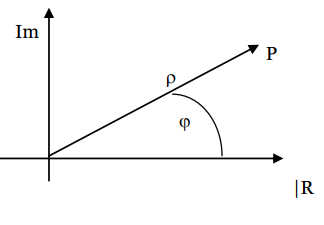
\includegraphics{../../../Imagenes/Superior/Complejos/Complejos02.PNG}
\\
\large Relación entre forma binomica y polar.
\normalsize
\\
\\
Por pitagoras es muy sencillo encontrar la siguiente relación:
\begin{align}
  a &= \rho \cos(\varphi)\\
  b &= \rho \sin(\varphi)
\end{align}
Esto es util si se quiere pasar de polar a binomica ya que tenemos despjeados los valores de $a$ y $b$ en función de $\rho$ y $\varphi$. Veremos ahora como pasar de binomica a polar. Con un poco de pensamiento llegamos a:
\begin{align}
  \rho &=\sqrt{a^{2}+b^{2}}\\
  \varphi &= \arctan(\frac{b}{a})
\end{align}
Estas formulas se deducen sencillamente con algunas propiedades de trigonometria y sin duda son ciertas y muy utiles pero, para algunos casos especiales, hay que pensar un poco mas.
\\
Por ejemplo, ¿Qué pasa si $a=0$ ? Entonces el numero es imaginario puro, ya que $a$ es la parte real. Los numeros imaginarios puros se encuentran sobre el eje imaginario (o eje de ordenadas) es decir, su argumento será de $\frac{\pi}{2}$ o bien $3\frac{\pi}{2}$ dependiendo de su signo.
\\
Pero aún hay un problema, la función $\tan(x) = y$ no es biyectiva en todo el dominio y por lo tanto se utiliza con el dominio reestringido a $(-\frac{\pi}{2};\frac{\pi}{2})$ para que exista su inversa $\arctan(x)=y$. Y todo esto, ¿Qué significa? Pues que la función de $\varphi$ en la calculadora sirve para calcular valores entre $(-\frac{\pi}{2};\frac{\pi}{2})$, es decír, complejos en el primer y cuarto cuadrante. Con un poco de pensamiento podemos solucionar esto solo sumando $\pi$ al valor cuando sabemos que nuestro numero está en el segundo o tercer cuadrante.


Veremos un ejemplo para clarificar todo este palabrerio. Escribamos en polar el siguiente numero: $-1 + i \sqrt{3}$
\\
Primero que nada notemos que como $a$ es negativo y $b$ positivo, sabemos que el numero se encuentra en el segundo cuadrante.
\\
Ahora calculemos el modulo que es bastante sencillo:
$$
\rho =  \sqrt{(-1)^{2} + (\sqrt{3})^{2}} = 2
$$
Ahora usamos la formula del argumento y vemos que obtenemos:
$$
\varphi = \arctan(-\sqrt{3}) = -\frac{\pi}{3}
$$
\\
Pensamos un poco y nos damo cuenta que un argumento de $-\frac{\pi}{3}$ deja el complejo en el cuarto cuadrante, pero el complejo original se encontraba en el segundo.

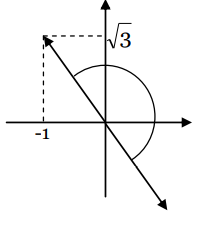
\includegraphics{../../../Imagenes/Superior/Complejos/Complejos03.PNG}
\\
Aquí se nota porque se debe sumar $\pi$ o medio giro para obtener el argumento del complejo original. Y nuestro complejo queda:
$$
z = [2 ; 2\frac{\pi}{3}]
$$
\\
\huge Forma trigonometrica de un complejo.
\normalsize
\\
\\
$$
z = \rho (\cos\varphi + i \sin\varphi)
$$
En esta formula se esconden todas las relaciones entre binomica y polar que vimos anteriormente. Pero además el famoso matemático Euler demostró:
$$
\rho e^{i\varphi} = \rho (\cos\varphi + i \sin\varphi)
$$
No entraremos en detalle sobre la demostración de esta formula, pero recomiendo fuertemente buscar información al respecto porque la demostración es una de las mas bellas de las matematias. Para la materia solo la tomaremos como verdadera y diremos que la forma exponencial de un numero complejo $z$ es $\rho e^{i\varphi}$ donde $\rho = |z|$ y $\varphi = \arg(z)$. De aquí además es de donde sale la bella identidad: $e^{i\pi} + 1 = 0 $ ya que $-1$ tiene modulo $1$ y argumento $\pi$.
\\
\\
\huge Operaciones en forma polar.
\\
\\
\Large Igualdad
\normalsize
\\
\\
Sea $z_1=[\rho_1;\varphi_1]$ y $z_2=[\rho_2;\varphi_2]$
$$
z_1 = z_2 \Leftrightarrow \rho_1 = \rho_2 \hspace{5pt} \wedge \hspace{5pt} \varphi_1 = \varphi_2 + 2k\pi
$$
Para que dos complejos sean iguales deben tener el mismo modulo y sus argumentos pueden diferir en una cantidad entera de giros $(2\pi)$.
\\
\\
\Large Multiplicación
\normalsize
\\
\\
Sea $z_1=[\rho_1;\varphi_1]$ y $z_2=[\rho_2;\varphi_2]$
$$
z_1 \cdot z_2 = [\rho_1 \cdot \rho_2 ;\varphi_1 + \varphi_2 ]
$$
Esta formula de la multiplicación quizas no tenga sentido a primera vista, por eso realizaremos la demostración:
$$
z_1 = \rho_1e^{i\varphi_1} \hspace{5pt} \wedge \hspace{5pt} z_2 = \rho_2e^{i\varphi_2}
$$
$$
\rho_1e^{i\varphi_1} \cdot \rho_2e^{i\varphi_2} = (\rho_1 \cdot \rho_2) \cdot (e^{i\varphi_1}\cdot e^{i\varphi_2}) = (\rho_1 \cdot \rho_2) \cdot e^{i(\varphi_1 + \varphi_2)} = [\rho_1 \cdot \rho_2 ;\varphi_1 + \varphi_2 ]
$$
\\
\\
\Large División
\normalsize
\\
\\
$$
\frac{z_1}{z_2} = [\frac{\rho_1}{\rho_2 };\varphi_1 - \varphi_2 ]
$$
La demostración es muy parecida a la anterior y ya se puede ver a simple vista.
\\
\\
\Large Potencias naturales en forma Polar.
\normalsize
\\
\\
Con $n \in \mathbb{N}$
$$
z^{n} = [\rho^{n}; n\cdot\varphi]
$$
Esta formula se puede deducir sencillamente reflexionando sobre la demostración de la multiplicacion presentada anteriormente.
\\
\\
\Large Raiz n-ésima.
\normalsize
\\
\\
Como vimos, en la forma binomica solo es posible calcular raices cuadradas, o en su defecto, raices potencias de $2$ ya que estas pueden descomponerse en raices cuadradas. Gracias a lo forma polar podemos resolver raices n-ésimas de un complejo.
\\
Sea $ z = [\rho;\varphi]$ y $ w = [r;\theta]$ una raíz n-ésima de z tal que $w^{n} = z$.
Entonces se deduce:
$$
w^{n} = z \Rightarrow [r^{n};n\theta] = [\rho;\varphi]
$$
Y por igualdad de complejos:
\begin{align}
  r^{n} &= \rho\\
  n\theta &= \varphi +2k\pi \\
\end{align}
\\
\begin{align}
  r &= \sqrt[n]{\rho}\\
  \theta &= \frac{\varphi+2k\pi}{n}
\end{align}
Finalmente, con $ 0 < k < n-1$: 
$$
w_k = [\sqrt[n]{\rho};\frac{\varphi+2k\pi}{n}]
$$
\\
Importante: cuando $k=n$ obtenemos $w_0$, por eso  $k$ va de $0$ a $n-1$, luego empiezan a repetirse. Además, por convención, antes de calcular raices n-ésimas se escribe al complejo en su primer giro positivo. De esta forma, las raices quedan ordendas a partir del semieje positivo real en sentido positivo (antihorario).
\\
\large Representacion geometrica
\normalsize
\\
\\
Como $|w_k|$ no depende de $k$ entonces:
$$
|w_0| = |w_1| = |w_2| = |w_{n-1}| = \sqrt[n]{\rho}
$$
Entonces los afijos de todas las raices están sobre la circunferencia de radio $\sqrt[n]{\rho}$.
\\
Además, la distribución será equiespaciada, ya que el argumento (ángulo) aumenta en $k\cdot \frac{2\pi}{n}$. Es decir un entero por una fracción de giro que depende de $n$. Esto secciona el giro completo en $n$ partes iguales.
Para resumir podemos decir que los afijos constituyen los vertices de un polígono regular de $n$ lados inscripto en la circunferencia de radio $\sqrt[n]{\rho}$ centrada en el origen.
\\
\\
Ejemplo: la grafica de las $ \sqrt[3]{-8i}$

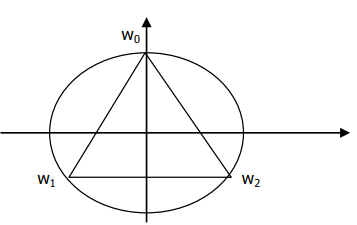
\includegraphics{../../../Imagenes/Superior/Complejos/Complejos04.PNG}
\\
\\
\Large Raices primitivas de la unidad.
\normalsize
\\





\end{document}